\chapter{Progettazione}
La fase di progettazione prevede principalmente la scelta dell'architettura da usare, su cui costruire il sistema. 
\\Dato il contesto di utilizzo dell'applicativo, la necessità principale è la sincronizzazione del lavoro dei dipendenti. L'obiettivo è quello di informare ogni dipendente del avvenimento di eventi a cui esso è interessato. Ogni azione deve essere memorizzata nel sistema, in conseguenza della quale esso provvede ad avvisare il gruppo di dipendenti relativo.
\\Ad esempio, al momento della registrazione di un'ordinazione da parte di un cameriere, il sistema provvede a notificare lo chef/pizzaiolo (realizzatore in generale) per informalo della nuova pietanza da preparare.
\\Per identificare l'architettura ideale bisogna elencare quali sono i componenti che ne fanno parte e in che modo sono interconnessi.
\begin{itemize}
	\item I componenti sono di due tipologie:
		\begin{itemize}
			\item Dispositivi utente, rappresentano i dispositivi fisici concessi ai dipendenti (smartphone o applicazione desktop)
			\item Sistema centrale, racchiude la logica di gestione e a cui i dispositivi utente possono fare accesso.
		\end{itemize}
	\item I connettori sono principalmente protocolli di rete, in quanto il sistema è pensato anche per dipendenti che hanno la possibilità di spostarsi all'interno del locale e accedere al sistema centrale in modalità remota.
\end{itemize}
Alla base di ciò i componenti devono ricevere dei cambiamenti del sistema tramite opportune \textit{notifiche}, evitando quindi attese attive.

\section{Architettura}
Sulla base delle necessità descritte in precedenza, si è scelto di utilizzare uno stile architetturale del tipo \textbf{Publish-Subscribe}. Per la realizzazione dell'applicativo infatti vengono ripresi tutti i vantaggi dello stile a \textit{invocazione implicita}:
\begin{itemize}
	\item \textit{Disaccoppiamento spaziale}: tutti i componenti sono altamente disaccoppiati, favorendo la scalabilità del sistema. Il proprietario può quindi assumere un numero di dipendenti variabile senza conseguenze.
	\item \textit{Disaccoppiamento di sincronizzazione}: tutti i componenti non lavorano in "polling", ovvero in attese attive che possono bloccare il sistema.
	\item \textit{Disaccoppiamento temporale}: tutti i componenti possono essere volatili nel sistema.
\end{itemize}
In relazione ai componenti descritti, tutti i dipendenti sono dei \textit{Subscribers} mentre il sistema centrale è l'unico \textit{Publisher}.
\\I dipendenti, effettuando l'accesso, si iscrivono in automatico al Publisher.
Dato che il sistema può contenere un numero notevole di dipendenti, il Publisher fa uso di \textbf{Proxy} per smistare i messaggi solamente a specifici Subscribers.
\\Essi infatti all'atto del login non conoscono i Proxy del sistema, ma è il sistema stesso che li racchiude in gruppi (con lo stesso ruolo) e li associa a determinati Proxy. Tutto ciò si traduce in una distribuzione più efficiente del calcolo computazionale.
\\Riassumendo quindi:
\begin{table}[H]
	\centering
	\begin{tabular}{|l | p{0.75\linewidth} |}
		\hline
		\textbf{Componenti} & Publisher, Subscribers, 
		Proxy \\
		\hline
		\textbf{Connettori} & Protocolli di rete \\
		\hline
		\textbf{Dati} & Notifiche, Richieste di informazioni, Informazioni pubblicate \\
		\hline
		\textbf{Topologia} & Subscribers sono connessi al Publisher indirettamente, ricevendo e inviando notifiche attraverso i Proxy \\
		\hline
		\textbf{Vantaggi} & Subscribers sono tutti disaccoppiati lavorando in parallelo. Le notifiche vengono ben distribuite grazie ai Proxy \\
		\hline
		\textbf{Svantaggi} & Il controllo computazionale è caricato tutto sul sistema centrale. Nessuna conoscenza di quali componenti risponderanno ad un eventi \\
		\hline
	\end{tabular}
\end{table}

\subsection{Main System}
Il sistema principale è l'unico Publisher dello stile utilizzato. Studiando i vari stili architetturali, tra quelli visti durante il corso, l'architettura del sistema non si rispecchia in uno stile architetturale ben preciso, ma è caratterizzata nel seguente modo:
\begin{figure}[H]
	\centering
	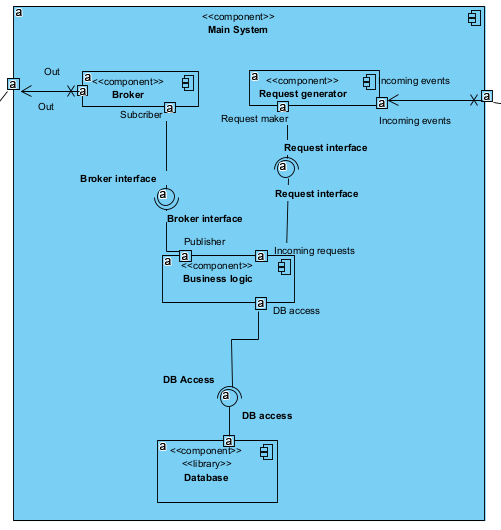
\includegraphics[width=0.4\textwidth]{Immagini/main_system.png}
\end{figure}
\begin{itemize}
	\item \textbf{Database}: Al livello più basso, il componente, racchiude tutte le funzionalità per accedere e modificare i dati all'interno della base di dati del sistema. La business logic accede al database solo attraverso all'interfaccia che tale livello offre, mascherando la reale implementazione.
	\item \textbf{Business Logic}: Al livello centrale, il componente, racchiude tutte le funzionalità per manipolare le richieste e i dati del sistema. Effettua tutti i controlli necessari prima di inviare una risposta. Si occupa principalmente di implementare i casi d'uso.
	\item \textbf{Broker}: Al livello più alto il Broker si occupa solo di inviare i le risposte (prodotte dalla Business Logic) ai diretti interessati. 
	\item \textbf{Request Generator}: Al livello più alto esso riceve, e identifica, le richieste dall'esterno e le inoltra alla Business Logic che si occupa di elaborarle e inviare le risposte al Broker.
\end{itemize}
La Business Logic deve esporre un'interfaccia al Request Generator che contiene le funzioni in relazione al caso d'uso da realizzare.

\subsection{Proxy}
Il proxy contiene un'insieme di utenti connessi al sistema tramite applicazione. Esistono più proxy, ognuno associato ad una categoria di utenti (i.e. Proxy Camerieri è associato a tutti i camerieri). Così facendo, all'atto dell'invio di un messaggio il Broker lo invia ad un relativo Proxy che provvede a smistarlo correttamente. 
\begin{figure}[H]
	\centering
	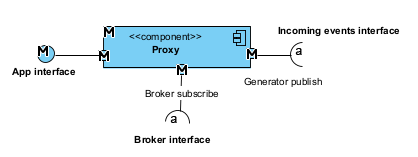
\includegraphics[width=0.6\textwidth]{Immagini/proxy.png}
\end{figure}
Oltre a inviare i messaggi a tutti i dispositivi associati, esso riceve anche informazioni solo da essi.
\\Esso è quindi dotato di tre interfacce:
\begin{itemize}
	\item Un'interfaccia per collegarsi al Broker. Il Broker invia un evento da pubblicare, il proxy lo pubblica a tutti i suoi dispositivi.
	\item Un'interfaccia per collegarsi al Request Generator. Il proxy riceve dai dispositivi eventi di richiesta, il Request Generator riceve da esso l'evento da elaborare.
	\item Un'interfaccia per collegarsi all'applicazione mobile.
\end{itemize}

\subsection{Applicazione Mobile}
Tutto il calcolo computazionale è a carico del \textit{Main System}, mentre lo smistamento dei messaggi è a carico dei \textit{Proxy}. L'applicazione deve solo ricevere e inviare eventi dal proxy (o dai proxy, se più di uno) associato. La costruzione del messaggio avviene tramite un'interfaccia grafica per ogni contesto, il resto è gestito tutto dal Main System.
\\A tal proposito si è utilizzato il pattern Architetturale \textit{MVC (Model View Control)} per la realizzazione dell'applicazione.
\begin{itemize}
	\item \textit{Modello} contiene tutti i dati necessari per il messaggio da inviare o ricevuto dall'esterno.
	\item \textit{Controllo} contiene tutte le funzionalità per interfacciarsi all'esterno tramite opportuni protocolli di rete per inviare e ricevere messaggi.
	\item \textit{View} è la rappresentazione grafica dei dati.
\end{itemize}



\subsection{Component Diagram}
\begin{figure}[H]
	\centering
	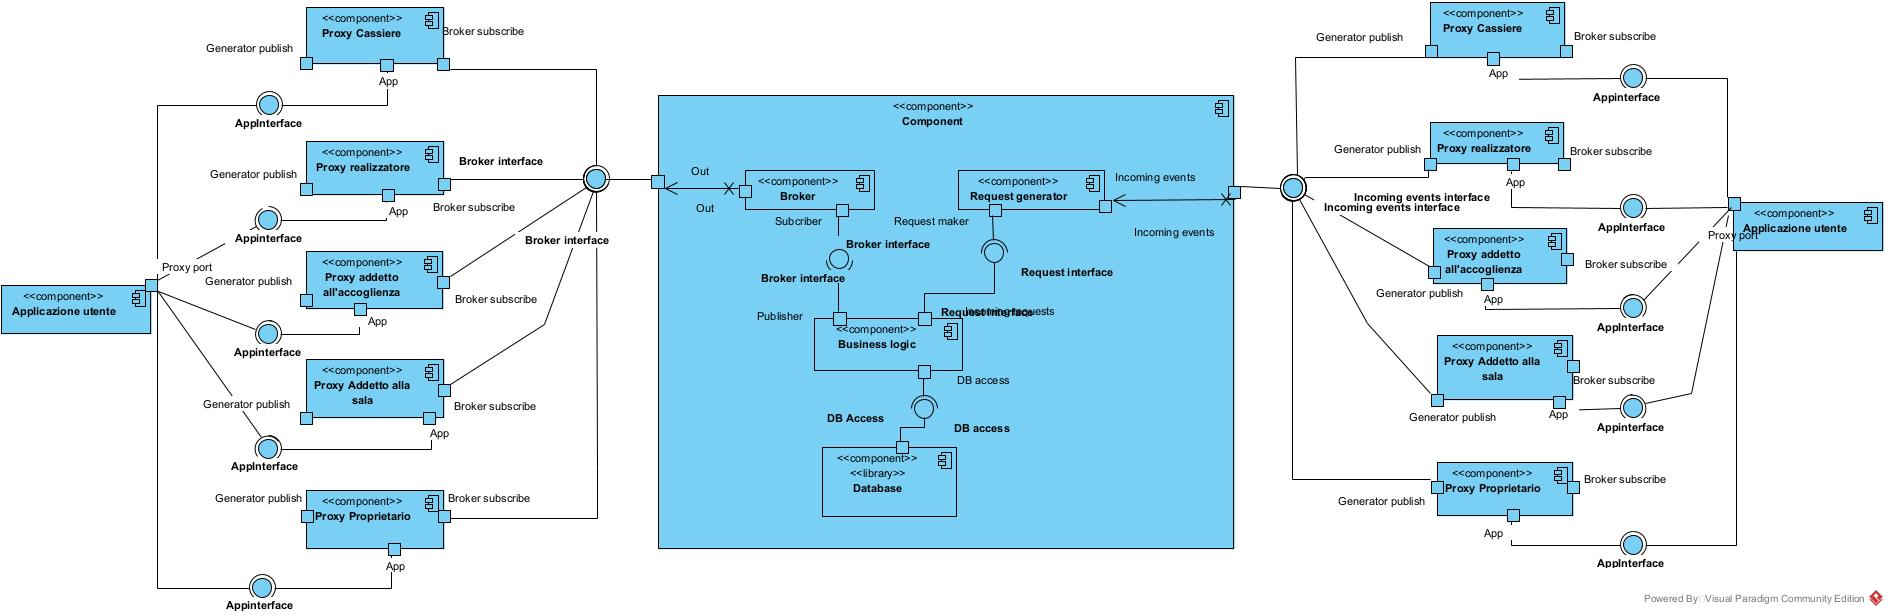
\includegraphics[width=1\textwidth]{Immagini/dynamic components.jpg}
\end{figure}

\section{Database}
Il database deve contenere le informazioni di base che devono essere utilizzate, a partire dai dipendenti che vengono registrati nel sistema e finire con le ordinazioni che vengono effettuate durante l'utilizzo del sistema.
\begin{figure}[H]
	\centering
	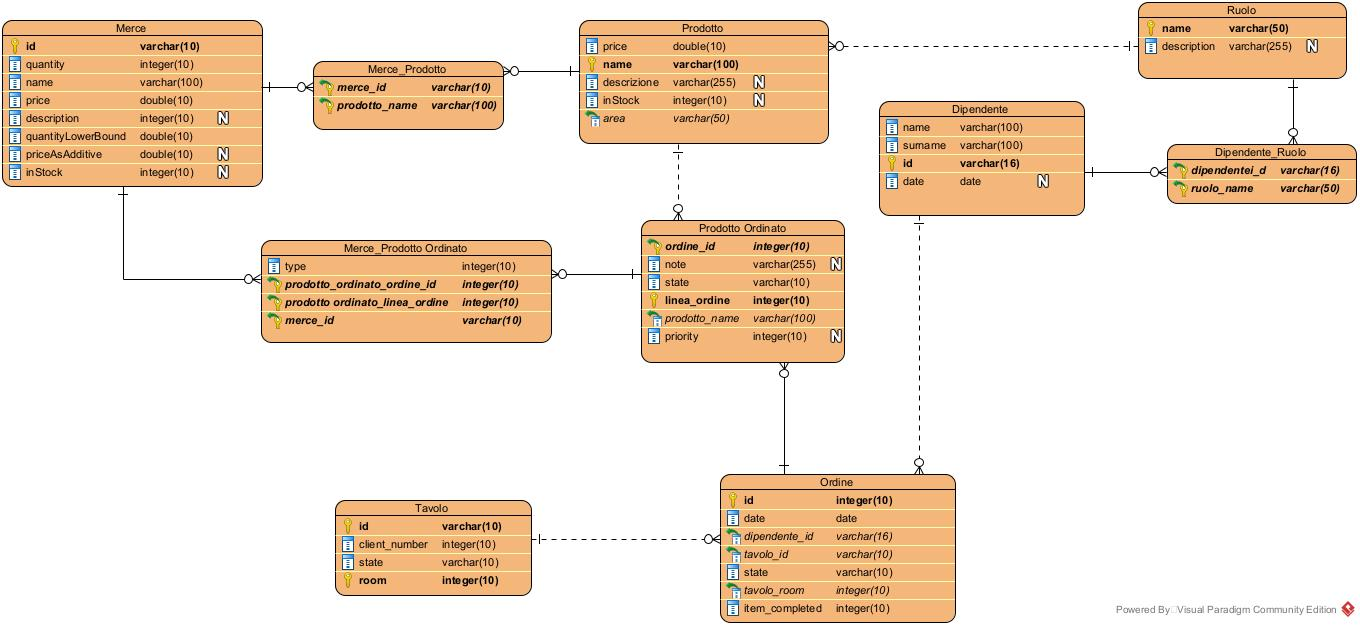
\includegraphics[width=1\textwidth]{Immagini/database.jpg}
\end{figure}
Le caratteristiche principali del database sono le seguenti:
\begin{enumerate}
	\item Le merci hanno, oltre alle informazioni di base quali prezzo, codice identificativo, nome, etc, hanno un attributo \textit{priceAsAdditive}. Tale attributo, se non nullo, indica il prezzo da aggiungere se quella merce è usata come merce aggiuntiva di un prodotto.
	\item Il \textit{Prodotto Ordinato} è un'associazione ternaria tra \textit{Ordine}, \textit{Prodotto} e \textit{Merce}.
	 \item Ogni prodotto ha un attributo collegato all'entità \textit{Ruoli}. Esso serve per indicare a che attività appartiene quel prodotto.
\end{enumerate}
Il precedente database si riferisce solo ai casi d'uso che si sono scelti di implementare. Non contiene, ad esempio, la gestione delle vendite e lo storico del locale.

\section{Deployment Diagram}
\section{Class Diagram}
\section{Sequence Diagram}